
\chapter{Background and Theory}

The goal of this work is the electrical characterization of Si and SiGe core fibers produced by the molten core fiber drawing method. This chapter gives an introduction to the molten core fiber drawing method and laser treatment used to produce the fibers. The  crystallinity and composition of SiGe alloy fibers obtained by these methods is then discussed. Electrical measurements on fiber cores is introduced including the principles of metal semiconductor contacts, four point probe electrical measurements and effects of finite contact sizes. %Lastly the principles behind other characterization techniques used in this study are given. 

\section{Fiber Fabrication}
\subsection{Molten Core Fiber Draw}
\begin{figure}[H]
    \centering
    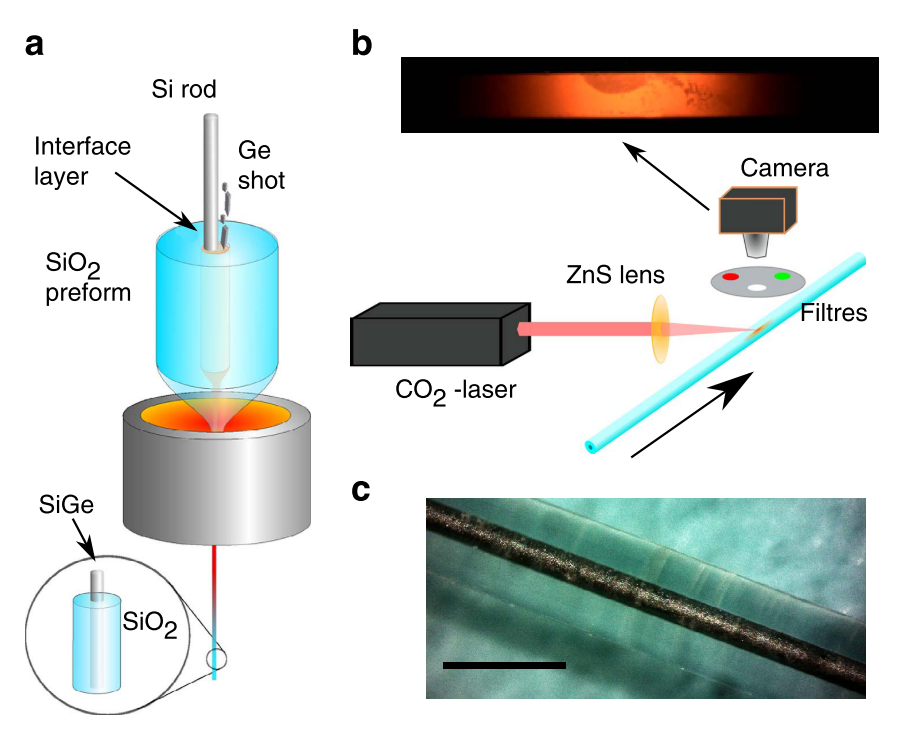
\includegraphics[width=.8\textwidth]{fig/intro-background/MCD.png}
    \caption{Caption\cite{Coucheron2016}}
    \label{MCD}
\end{figure}

The use of the MCD techniques to produce Si core fibers is first attributed to the work of Ballato \cite{Ballato2008SiliconFiber} in 2008. This showed the possibility of producing semiconductor optical fibres with a method that could scale to produce commercially relevant lengths. The MCD method uses a silica preform that acts as a crucible and is filled with the desired core material. Using a commercial draw tower, the preform is heated above the softening temperature of the glass and melting point of the core phase and is drawn into a fiber; illustrated in figure \ref{MCD}. The drawing rate is on the order of meters per minute. The MCD involves high temperatures and liquid phase chemistry which allows for interaction between the core and cladding and leads to the dissolution of oxygen into the core. This reactivity during the draw can also exploited to produce fibers with a different core phase than the original starting material \cite{almuminium core}. The introduction of the alkaline earth oxide CaO as an interface modifier  \cite{Nordstrand2013AlkalineProduction} marked a turning point in the MCD method. This allowed for fibers to be produced with negligible oxygen content and helped to reduce stress in the fiber originating from the mismatch between the coefficients of thermal expansion between the core and cladding. Typical fibers showed poly-crystalline cores and high transmission losses. This led to $\text{CO}_2$ laser post processing of the fibers and single crystalline Si cores \cite{Healy2016Loss}. It was also found that structures could be written into the core and bandgap modified in Si fibers \cite{Fokine2017LaserFibers, Healy2014ExtremeFibres} and compositional variation could be written in SiGe fibers \cite{Coucheron2016}.



\subsection{As-drawn and Laser Annealed SiGe fibers}

\begin{figure}[t]
    \centering
    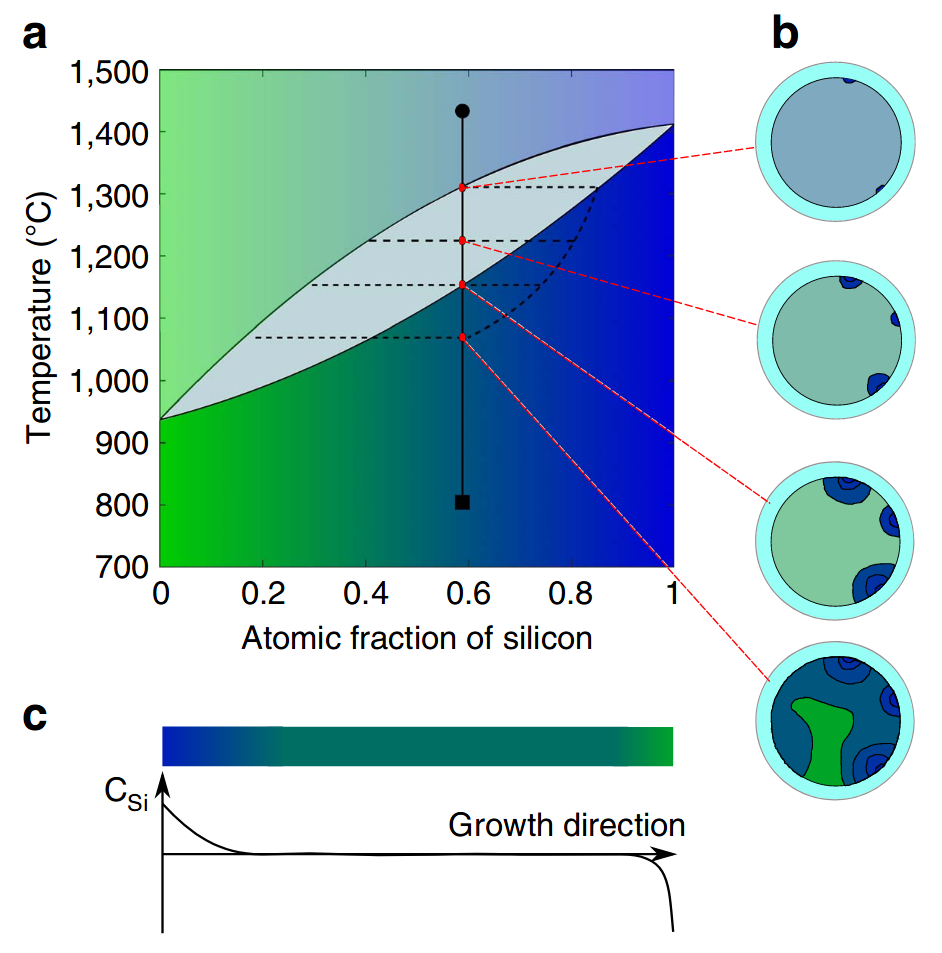
\includegraphics[width=.7\textwidth]{fig/intro-background/coucheron.png}
    \caption{Figure and caption from \cite{Coucheron2016}}
    \label{sige_phase}
\end{figure}
The equilirium phase diagram for the SiGe system is show in figure \ref{sige_phase}. Due to the large separation between the solidus and liquidus phases, as the fiber cools Si rich areas are first to solidify leaving a Ge rich melt. This process leads to variations in composition with the last areas to solidify being Ge rich. This process occurs across the fiber cross section (figure \ref{sige_phase} b) and along the fiber axis (figure \ref{sige_phase} c) with transverse grains ending in Ge rich areas. Nucleation is thought to occur at the the fiber cladding, and either single and multiple grains can span the fiber cross section \cite{Coucheron2016}. The work of Coucheron et. al \cite{Coucheron2016} showed that with  6 at\% Ge and $\SI{130}{\micro\meter}$ core diameter, fibers were found to have a single grain across the fiber cross section with grain lengths likely on the $\si{\mm}$ scale. 

\subsection{Laser annealed SiGe fibers}
As grain boundaries and compositional variation increase scattering, re-crystallization of the core is performed by laser annealing to achieve a homogeneous composition (figure \ref{MCD} b). A $\text{CO}_2$ laser is used with emission in the infrared (IR). The IR radiation is absorbed by the glass and the core is melted by convection. A melt zone is established across the diameter core and the fiber translated across the laser to move the melt zone along the fiber length. This method produces high temperature gradients and allows for a rapid solidification front creating single crystalline cores with homogeneous composition \cite{Coucheron2016}. It is thought that the high velocities suppress polycrystalline growth as, as stable nuclei have little time to form and grow ahead of the advancing growth front \cite{Coucheron2016}.  



%MCD of SiGe fibers produces a core with variations in composition. 
%The method has been used to produce silicon fibers with a sharp interface and negligible low 02 content. Alloy %fibers follow solidification (cite the paper here and maybe include the diagram on SiGe fibers?) 
%Crystalization is done by laser annealing ...describe here cite same paper. XRD diffraction and tomography can be performed, is able to show transvegrain boundaries across the fiber scanning along the fiber can show . 
%crystalization during fiber drawing:
%\cite{Balci2019FiberAnalysis}

% Ursula These are the samples and this is what we want to look at. Experiments performed what and why

%\section{SEM and EDS}
%\section{Deposition}
%\section{Lithography}

%\section{Ohmic Contacts}
%\subsection{Silicide Technology}
%Silicide self alligned layers (salicides) are the dominant industry method for creating ohmic contacts to semiconductor devices. This is due to the metal-like resistivity of silicides and their stability at high temperatures. Common silicides used in the industry are TiSi, WSi, CoSi and NiSi. Of these NiSi has the lowest formation temperature.


\section{Resistivity and Metal Semiconductor Contacts}
The band diagram of Si is shown in figure \ref{si_band}. The band structure of crystals arises from the overlapping electron wave functions, which creates continuous "bands" of allowed energies. Semiconductors are defined as having a bandgap, that is a range of forbidden energies splitting the band diagram into a valence and conduction band. In an intrinsic crystal the valence band is full, meaning there are no available free states. Energy equal to or greater than the bandgap energy is required to move an electron to the conduction band to allow current to flow. By introduction of a dopant, that is an atom with one more or less valence electron, energy states are introduced very close to the conduction or valence band. Thermal energy is sufficient to allow electrons to move to or from these states creating free charge carriers, i.e. holes in the valence band and electrons in the conduction band. A metal is defined as having half filled or overlapping bands with a continuum of available states above the Fermi Energy. The work function of a metal ($\phi_m$) or semiconductor ($\phi_s$) is the energy difference between the vacuum energy and the fermi level. For semiconductors the electron affinity, $\chi_s$ is more commonly used and is defined as the difference between vacuum energy and the bottom of the conduction band $\chi_s = E_{vac}-E_c$.

\subsection{Schottky junctions}

\begin{figure}[h]
 %h here H requires float, exactly here, h! overide latex
\centering
\begin{subfigure}{.5\textwidth}
  \centering
  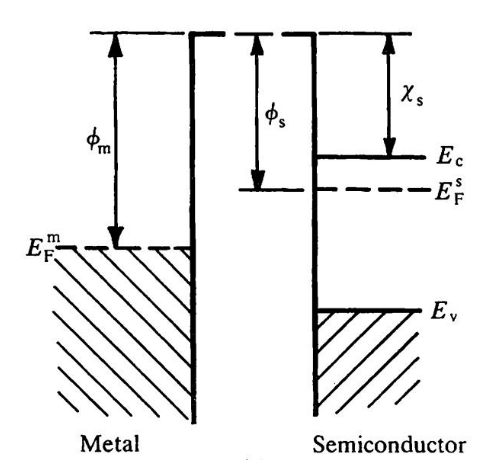
\includegraphics[width=\linewidth]{fig/intro-background/metal-semi_1.png}
  %\caption{1a}
  \label{shottky_a}
\end{subfigure}% %blank line makes figures vertical
\begin{subfigure}{.5\textwidth}
  \centering
  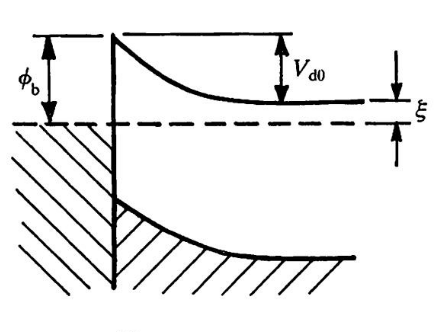
\includegraphics[width=\linewidth]{fig/intro-background/metal-semi_2.png}
  %\caption{1a}
  \label{shottky_b}
\end{subfigure}% %blank line makes figures vertical
\label{schottky}
\caption{Figure reprinted from \cite{RhoderickMetal-SemiconductorEDITION}}
\end{figure}


Current-Voltage (I-V) and hall measurements typically require metal-semiconductor junctions, which introduce distortion or "bending" to the semiconductor band energies. This leads to non-ohmic I-V characteristics and current rectification.  Figure \ref{schottky} a shows a the energy levels of a metal and n-type semiconductor in relation to the vacuum energy. When the metal and semiconductor come into contact (figure \ref{schottky} b) come into contact, the Fermi energies align as higher energy electrons move into empty states in the metal. The charge the has transferred to the metal is balanced by an area of positive charge on the semiconductor composed of the positively charged ionized dopants. This area is called a space charge region, or depletion region and has a width that depends on on the dopant density. This arrangement is called a schottky contact and has rectifying properties. The barrier height is defined as $$\phi_b = \phi_m - \chi_s$$. Under forward bias, that is negative potential on the semiconductor, the semiconductor bands are raised, and the barrier is lower for electrons to move into the metal. This leads to an increasing current with increasing voltage. Under reverse bias the barrier seen is $\phi_b$ and only a small constant current can flow that is orders of magnitude smaller than under forward bias. This leads to the rectifications properties of a Schottky junction \cite{KasapS.O2002Poem}.

\subsubsection{Ohmic Contacts}

In theory near-ohmic contacts can be achieved by choosing a metal whose work function is less than the work function of the semiconductor for n-type semiconductors and greater than the work function of the semiconductor for p-type semiconductors. In practice surface states which arise due to an interruption in the perfect crystal lattice can lead to fermi level pinning and it is no longer possible to predict the barrier height from the work function of the metal \cite{D.K.Schroder2006MATERIALEdition}. In practice other methods are typically used to achieve ohmic contact, the most common being heavy doping of the junction or the use of silicides. For example Al is a  p-type dopant for silicon. Annealing an Al contact on n-type silicon will create a heavily doped region beneath the contact. This in turn narrows the depletion region and allows for tunneling through the barrier between the metal and semiconductor. Another common mechanism important in industry is the use of silicide contacts, due to their stability, low formation temperatures and small barrier heights. Ni,Ti,W and Co are all common metals used for silicide contacts with Nickel silicide forming at the lowest temperature at $~300\si{\celsius}$ \cite{}. 


\section{Four Point Probe}

    %intro to resistivity 
    
    The four-probe technique is a method that allows for sensitive resistivity measurements by eliminating the resistance of the measurement probes and contacts. In a two point resistivity measurement the resistance is the sum of the resistance of the leads, the resistance of the contacts and the resistance of the sample. %[current spreading etc, semicondutor devices]
    When the resistance of the leads and contacts becomes comparable to the sample resistance the method is no longer useful for accurately determining the resistance. The four-probe methods uses four contacts to the sample, two probes supply current to the sample and the voltage is measured across the remaining two probes. In the ideal case, due to their high impedance, no current flows through the voltage probes eliminating any contribution to the resistance due to the contacts and leads. Typical four-probes are designed to measure semiconductor wafers and thin films and consist of four co-linear Tungsten probes with constant spacing. While other geometries are possible %[citations]
    we will now consider this geometry for the following derivations. 
    

 
    For isotropic materials, electrical resistivity is a property that relates the current density in a sample to the electrical field applied to it. This gives the relation \begin{equation}
        \rho = \frac{E}{J}
    \end{equation}
    Experimentally it is the Resistance $R$ that is measured, which only defines a relationship between the current $I$ and the Voltage $V$ giving the familiar expression: \begin{equation}
        R = \frac{V}{I}
    \end{equation}
    
    In order to determine the resistivity of the sample, the geometry of the sample, and size and placement of the contacts must be known as these define the current paths within the sample. 
    
    \begin{figure}[h]
        \centering
        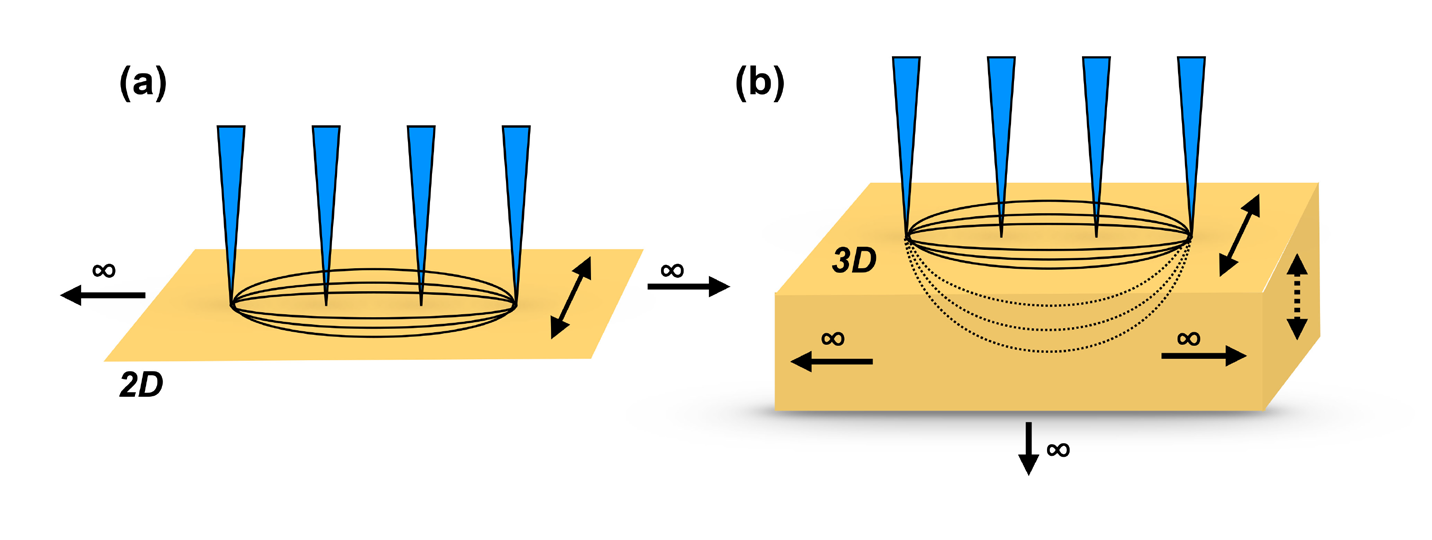
\includegraphics[width=0.7\textwidth]{fig/4pp/4pp_current.png}
        \caption{\cite{Miccoli2015TheSystems}}
        \label{fig:4ppcurret}
    \end{figure}
    For the case of the co-linear four point probe and a homogeneous sample, we can define the resistivity $\rho$ as:
    
    \begin{equation}
    \rho = F\frac{V_{2-3}}{I_{1-4}}
    \end{equation}
    where F is a correction factor that depends on the geometry of the sample and, the position of the contacts and their spacing \cite{Miccoli2015TheSystems}. Where the subscript denotes the probe numbers, e.g. $V_{2-3}$ refers to the voltage between probes 2 and 3. There are many works that derive the correction factor F for different sample geometries, thicknesses and probe positions \cite{Smits} \cite{ValdestResistivityTransistors} \cite{Topsoe1991GeometricCorrection} \cite{}. These solutions are found by using the method of images \cite{ValdestResistivityTransistors}, solving Laplace's equation \cite{Esposito2000DeterminationCrystals} and finite element methods \cite{Zimney2007CorrectionStudy} among others. 
    
    The simple cases of a semi-infinite volume and thin infinite sheet are solved without the use of boundary conditions by looking at the geometry of the current as it spreads into the sample. For a bulk specimen, infinite in all directions below a plane, the current will spread out from the source probes in hemispherical shells of equal current density \cite{Miccoli2015TheSystems}.
    The current density is given by $J=\frac{I}{2 \pi r^2_1}$ where $r_1$ is the radial distance from a source electrode. The electric field at this point is then given by:
    \begin{equation}
    E(r_1) = \rho J = \frac{\rho I}{2 \pi r^2}=\frac{-dV}{dr}
    \end{equation}
    Integrating both sides leads to an expression for the potential at this point. The measured potential can then by found by the difference in potential at the positions of the two inner probes. For the case of equidistant probes this gives the following expression:
    \begin{equation}
        \rho = 2 \pi s\frac{V}{I}
    \end{equation}
    
    For a 2D sheet of thickness $t \ll s$, current is confined in the direction normal to the plane and the current flow can by approximated by cylindrical shells with current density $J=2 \pi rt$. As the probe distance increases the number of possible current paths increases and directly cancels any increase in resistivity from the larger probe spacing, thus the resistance is independent of spacing and the resistivity is given by: 
    \begin{equation}
        \rho = \frac{\pi t}{ln2}\frac{V}{I}
    \end{equation}
  
  
\subsection{Fiber Geometry}
A Fiber with sufficiently large contact spacing can be treated as a wire. The resistivity of a wire is given by $\rho = \frac{L}{A}R$
where L is the length of the wire and A is the cross sectional area. The length L is the center to center spacing of the voltage contacts for the ideal case of high interface resistivity. The cross sectional area $A_t$ of the fiber can be derived as follows: \begin{align}
\Theta = \arccos{\frac{C}{D}}    \\
h = \sqrt{r^2-\frac{1}{2}C^2} \\
    A_t = \frac{\pi+2\Theta}{2\pi}*\pi r^2 + \frac{1}{2}Ch\\
\end{align}    
Where the variables are correspond to those in figure \ref{fig:fiber}.
When the fiber is polished past the mid point the cross sectional area $A_b$ is given by: \begin{equation}
    A_b = \pi r^2 -A_t
\end{equation}

\begin{figure}
    \centering
    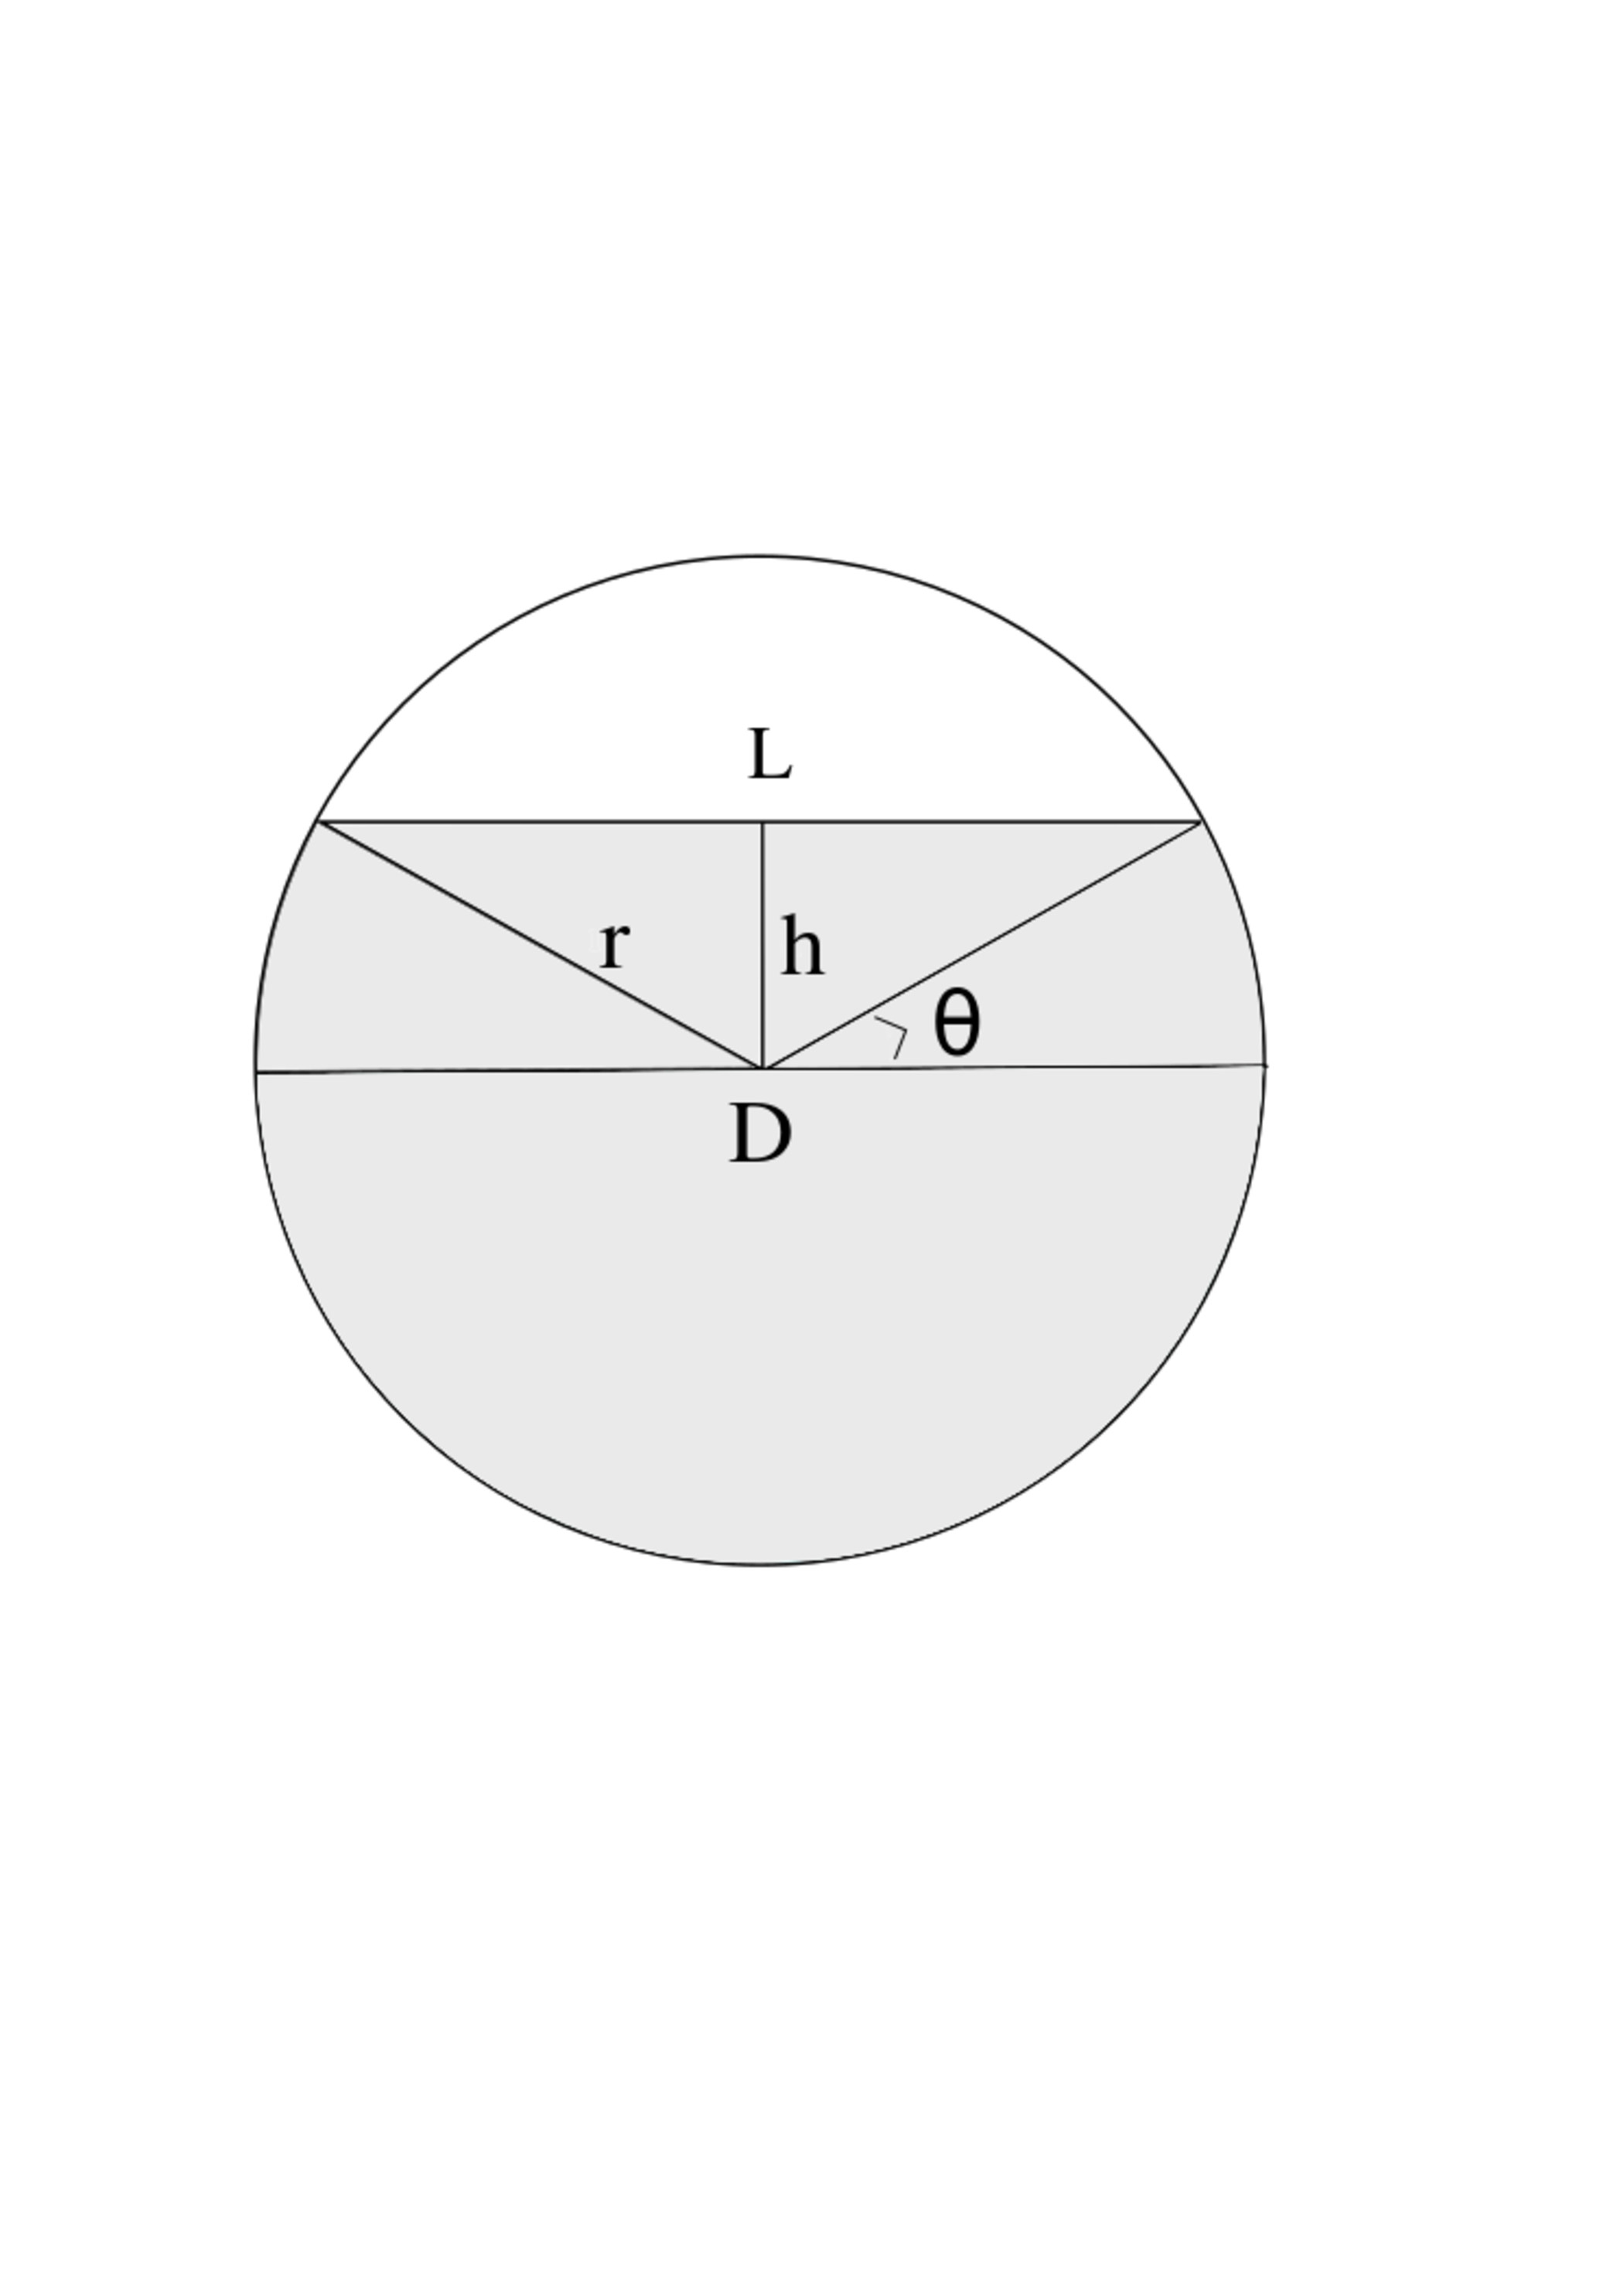
\includegraphics[width=.7\textwidth]{fig/polishing/fiberdiagram.jpg}
    \caption{Symbols used in the calculation of a fiber cross section, where the shaded area represents the remaining fiber area. Both L and D are subject to measurement errors.}
    \label{fig:fiber}
\end{figure}

  
    %correction for semicircular shape
    %correction for 
    \FloatBarrier
\section{Finite Size Contacts}
 The previous four point probe equations are derived for measurements made with ideal point like contacts and a high impedance voltmeter so that no current can flow through the contacts. In any real situation there will be a finite area of contact between the probe and the sample and finite interface resistance (also called contact resistance $R_c$) between the contacts and sample. This will allow current to flow into the contacts and will disturb the potential and current distributions in the sample \cite{Zimney2007CorrectionStudy}. With lithographically defined micro scale contacts this contact area may become large compared to the probe spacing, and the effects of the metal contacts must be considered. %here? 
 Two situations in this work required the use of small contact spacing. First is the occurrence of cracks with the fiber which limited the continuous length of fiber, and second is high resistivity fiber cores which require a small contact spacing in order to drive a measurable current through the sample without exceeding the voltage source range of the source meter unit. 
 
  
\begin{figure}[h]
  \centering
    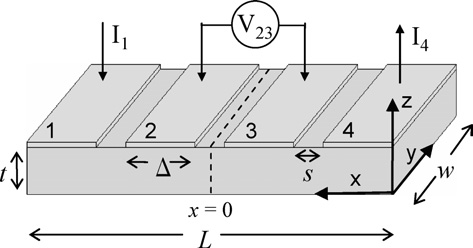
\includegraphics[width=0.5\textwidth]{fig/4pp/finite_size_contacts.png}
 \caption{Schematic of the co-linear 4-probe configuration with electrodes that span the width of the specimen. Figure and caption reprinted from \cite{Zimney2007CorrectionStudy}.}
\label{fig1}
\end{figure}

 Several theoretical and experimental studies have been done on the influence of finite size contacts for co-linear resistivity measurement \cite{Zimney2007CorrectionStudy}, \cite{Mak1989SpecificArsenide}, \cite{Ilse2014GeometricalMeasurements} \cite{Esposito2000DeterminationCrystals}. Zimney et al. and Mak et al. focus on rectangular contact bars and are most relevant for this analyses. Zimney et al has used finite element studies to investigate the influence of rectangular contacts spanning the width of a sample as shown in figure \ref{fig1}. These results may be applied to this work under the approximation that the semicircular fiber core cross section is rectangular. In this paper it is assumed that the resistivity of the contacts is much lower than the sample (the contacts are equipotential), the sample is homogeneous and that the contact resistance is ohmic.%talk about what defines interface resistivity. ohmic nonohmic elements. 
 
\begin{table}[b]
\begin{center}
    \begin{tabular}{|l|l|l|  }
    \hline
  
     The thickness ratio & $TR = \text{sample thickness} / \text{contact spacing}$ \\ 
     The electrode ratio & $ER =  \text{contact width}/\text{contact spacing}$ \\ 
     The interface resistance factor & $\alpha = \text{contact resistance} / \text{measured 4-probe resistance}$ \\
     \hline
    \end{tabular}
\end{center}
\caption{Dimensionless variables used in the analysis of Zimney et al. simplified for the case of an isotropic material \cite{Zimney2007CorrectionStudy}}
\label{dimensionless}
\end{table}
 
As the contacts span the sample width there is no current flow in the y direction (figure \ref{fig1}) and the analysis is equivalent to the two dimensional system. Several dimensionless variables describe the the geometry and are found in Table \ref{dimensionless}. The contact spacing $s$ is defined as the distance between the inner edges of the voltage sensing contacts. $R_m$ is the measured 4 terminal resistivity, $R_c$ is the interface resistance and $\Delta$ is the contact width. 

For the given geometry the resistivity is given by the following relation: 
\begin{equation}
    \rho   = F \frac{wt}{s}R_m = F \frac{wt}{s}\frac{V_{2-3}}{I_{1-4}}
\end{equation} 
where F is a correction factor accounting for any perturbation in the current distribution due to the influence of sample thickness and presence of contacts. Due to the definition of s is the distance between inner edges of the contact pads, F will not be equal to 1 for the case of a uniform current distribution. This is because the measured voltage will not be the voltage at the edge of the contact, e.g for $ER = 1$, $F = .5$.

%The correction Factor F for this geometry is solved by \cite{Esposito2000DeterminationCrystals}, for the condition of no influence of the contacts by solving Laplace's equation considering appropriate boundary conditions at the contact sample interfaces. 

 
 \begin{figure}[]
  \centering
    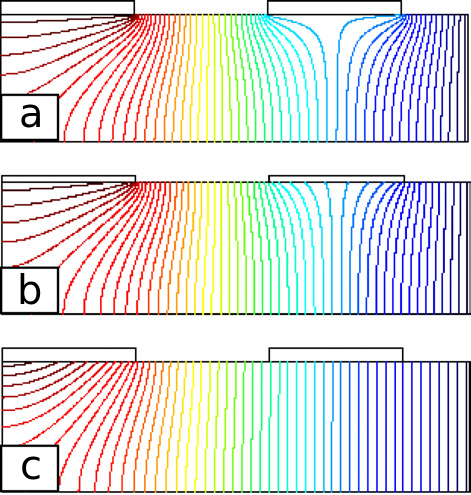
\includegraphics[width=0.5\textwidth]{fig/4pp/finite_contact_contour.png}
 \caption{ Potential contour plots for varying interface resistivity with $ER=1$ and $TR= 1$. The interface resistance increases from top to bottom: (a) \hspace{.5mm} $\alpha=0$, (b) \hspace{.5mm} $\alpha=0.1$ and (c) \hspace{.5mm} $\alpha>> 1$ . Figure and caption adapted from \cite{Zimney2007CorrectionStudy}.}
 \label{fig2}
\end{figure}


Figure \ref{fig2} illustrates the change in potential for varying contact resistivity for the case of $ER$ and $TR$ equal to one. The image shows half of a four point measurement where the left electrode is a current source, and the right electrode is a voltage sensing electrode. 

The influence of the contacts can be easily understood under two extremes of infinite or zero specific contact resistivity. With zero specific contact resistivity current will easily flow into the low resistivity contact pads, and the contact essentially short circuits the sample beneath. No potential drop occurs under the contact pad. With high specific contact resistivity, no current will flow through the contact, and the contact is isolated from the sample leaving the potential in the sample beneath unchanged \ref{fig1}(c). For intermediate values of contact resistivity a portion of the current will flow through the contact causing a potential drop across the contact-sample interface.
With these considerations it is shown that it is non-trivial  to determine the contact spacing that corresponds to the position in the sample of the measured potential. In the first case the potential in the contacts will be an average of the potential beneath the contacts \cite{Zimney2007CorrectionStudy} %more here?
and the the spacing is measured from the center of the contact, and the second case the measured potential is that of the sample at the edge of the contact, and the spacing is measured from the edge.


%what is important: order of magnitude of contact resistivity. How the correction factor changes. h
%$L = 3s + 4\Delta$

\begin{figure}[t]
  \centering
    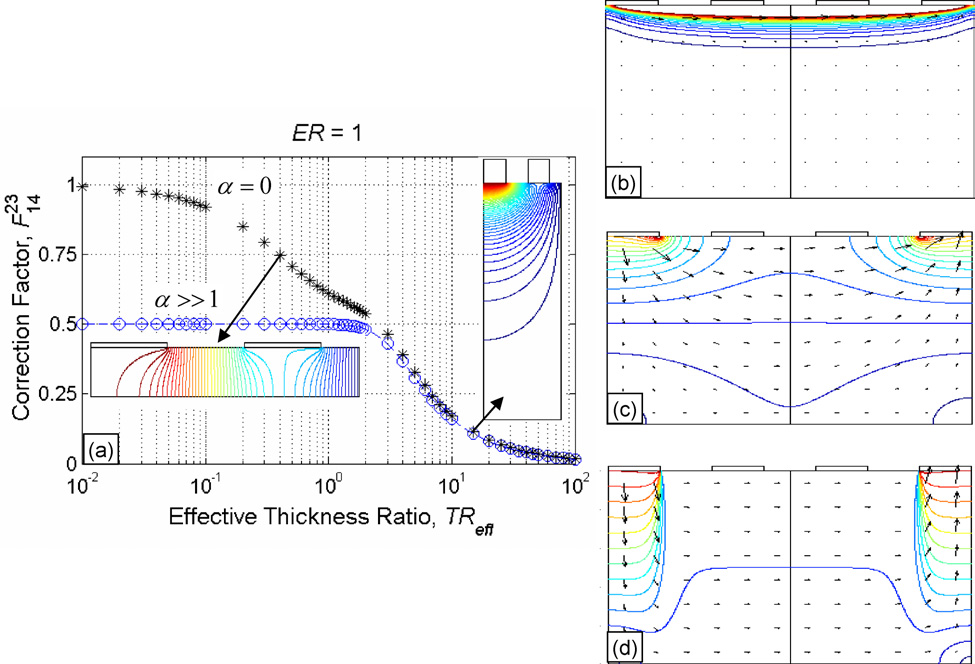
\includegraphics[width=\textwidth]{fig/4pp/ER1.png}
 \caption{  Figure and caption adapted from \cite{Zimney2007CorrectionStudy}.}
 \label{ER1}
\end{figure}


Figure \ref{ER1} a plots F against TR for the limiting cases of high and low contact resistivity ($\alpha = 0$ and $\alpha >> 1$ and with $ER = 1$ . The contour plots illustrate the potential field and current distribution (arrows) in the sample. The blue dashed line is an analytical solution derived in \cite{} for the case of high interface resistance. First looking at the case of high interface resistivity, where we only see the effects of thickness, we see F remains constant until $TR \sim 2$ where it begins to fall off sharply. This is explained by the current density no longer being constant throughout the thickness of the sample. When the thickness becomes large the current is confined to an area near the surface of the sample as illustrated in the \ref{ER1}(b), thus an increasing thickness causes a reduction in F. 
We see that for $\alpha = 0$ F approaches 1 for decreasing thickness. We see that as the TR decreases the equipotential created by the pads will have a greater influence through the depth of the sample until the electrodes become a short circuit to the sample. Larger electrodes will have a greater effect on the sample and thus the area where the cases converge will be shifted to higher values of TR. 

In this work it is important to know the point of divergence as the interface resistivity is in general an unknown. Using information on the typical core diameters of the measured fibers and the resolution of the lithography we can find the regime in which we need to worry about the correction factors. A fiber cross section will have a small area compared to a rectangular bar, and thus the current will be confined laterally and probe a larger depth; thus the point where F begins to fall off will be shifted to higher values of TR. Assuming an $\nicefrac{t}{s}$ of 1, we can safely achieve a $\Delta$ of $20\si{\micro\meter}$ with the MLA using MAN-440. Fiber cores in the study range from  $10-160 \si{\micro\meter}$ This gives $ $ between $0.5$ and $8$ which for a rectangular cross section is in the regime where the correction begins to become significant. Thus especially for the thinner fiber cores care must be taken to ensure a sufficiently large $\nicefrac{t}{s}$, and measured values must be treated as a bound to the actual value until an exact correction is derived for this geometry.  
\cleardoublepage